% Aneva est une grosse cruchasse =D

\documentclass[a4paper]{article}

\usepackage[utf8]{inputenc} 
\usepackage[francais]{babel}  
\usepackage[T1]{fontenc}

\usepackage{graphicx}

\usepackage[top=2cm, bottom=2cm, left=2cm, right=2cm]{geometry}

\usepackage{hyperref}

% Headers and footers:
\usepackage{fancyhdr}
\pagestyle{fancy}
          \fancyhf{}
          \fancyfoot[LE,RO]{\thepage}
          % Rulers width
          \renewcommand{\footrulewidth}{.3pt}
          \renewcommand{\headrulewidth}{.3pt}
\fancyhead[RO,RE]{Johann Chazelle, Elisa Abidh, Sandra Mondain}
\fancyfoot[LO,RE]{Compte-rendu du TP Sherlock}

\newcommand\PIXPATH{../ressources}

\title{\vfill \textbf{Compte-rendu du TP Sherlock}}
\author{Johann \bsc{Chazelle}, Elisa \bsc{Abidh}, Sandra \bsc{Mondain}}
\date{16 décembre 2010\vfill}

\begin{document}

\maketitle

\newpage

\section{Modèle de maintenance}
\begin{figure}[!h]
\begin{center}
        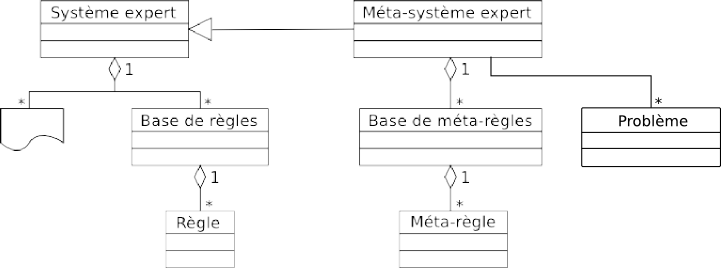
\includegraphics[width=500px]{\PIXPATH/Modele-Maintenance-2.png}
        \caption{Modèle de maintenance automatique de l'application Constat}
\end{center}
\end{figure}

\section{Réflexion sur la maintenance corrective et évolutive}
\begin{large}

\paragraph*{}
La maintenance corrective et évolutive d'une application informatique est en général nécessaire pour solutionner des problèmes qui n'avaient pas été envisagés au départ, et qui ne sont donc pas prévus dans la conception. \\
La maintenance évolutive permet donc d'allonger la durée de vie d'un logiciel en le complétant au fur et à mesure, au lieu d'en concevoir un nouveau plus complet. 

\paragraph*{}
Mettre en place une maintenance automatisée pour un logiciel permet de gagner du temps pendant les opérations de maintenance, car celles-ci sont effectuées plus rapidement de manière automatique avec l'aide de l'utilisateur, que par un développeur qui doit se "replonger" dedans, comprendre les spécifications du problème, etc. \\
La maintenance est également moins chère, car elle n'implique pas d'intervention (coûteuse) d'un développeur. \\
En revanche, la mise en place d'une maintenance automatisée coûte du temps et de l'argent pendant la phase de conception et de réalisation du logiciel. 

\paragraph*{}
En conséquence, il n'est pas toujours approprié de mettre en place un tel type de maintenance ; pour de petits logiciels qui auront peu besoin d'évoluer, ça n'apporte que peu, et c'est même au contraire du "gaspillage" de ressources (temporelles, humaines, financières). \\
Il faut donc se questionner avant (pendant la conception) sur les apports de la maintenance automatisée sur un projet spécifique, et comparer les coûts (en temps et en argent) de mise en place du système de maintenance par rapport aux coûts de la maintenance "manuelle" éventuelle sinon. 

\paragraph*{}
Bien sûr, la maintenance automatique ne peut pas résoudre tous les problèmes, mais seulement ceux pour lesquelles elle a été programmée, il y a donc une limite concrète à son efficacité et ses possibilités. On ne pourra donc pas résoudre des problèmes non prévus, ou ajouter de nouvelles fonctionnalités au logiciel. 


\end{large}






\end{document}